\documentclass[journal,twoside]{IEEEtran}

\usepackage{amsmath,amssymb,amsfonts}
\usepackage{algorithmic}
\usepackage{algorithm}
\usepackage{graphicx}
\usepackage{textcomp}
\usepackage{xcolor}
\usepackage{booktabs}
\usepackage{cite}
\usepackage{url}
\usepackage{microtype}
\usepackage{balance}
\usepackage{tikz}
\usetikzlibrary{shapes.geometric, arrows.meta, positioning, calc}
\usepackage{hyperref}

\hypersetup{
    colorlinks=true,
    linkcolor=blue,
    filecolor=magenta,      
    urlcolor=cyan,
    citecolor=blue
}

% Suppress all running header text (removes 'IEEE Access' and 'Kanth et al.')
\pagestyle{plain}
\makeatletter
\def\@oddhead{}
\def\@evenhead{}
\def\@oddfoot{\normalfont\footnotesize\hfil\thepage\hfil}
\def\@evenfoot{\normalfont\footnotesize\hfil\thepage\hfil}
\makeatother

\begin{document}

\title{AegisOne AI: An AI Copilot for Secure Web Application Development using Explainable Risk Analysis, Security Knowledge Graph, and Sandbox Validation}

\author{Praveen~Kanth~N,~\IEEEmembership{Student~Member,~IEEE},
        Sankavi~M,~\IEEEmembership{Student~Member,~IEEE},
        and~Vijayashree~J,~\IEEEmembership{Senior~Member,~IEEE}%
\thanks{Manuscript received October 15, 2026; revised October 28, 2026; accepted October 31, 2026. Date of publication November 2, 2026; date of current version November 5, 2026. This work was supported in part by the Department of Database Systems, School of Computer Science and Engineering, Vellore Institute of Technology (VIT), Vellore, Tamil Nadu 632014, India.}%
\thanks{Praveen Kanth N (Reg. No. 23MIC0078) and Sankavi M (Reg. No. 23MIC0126) are with the School of Computer Science and Engineering, Vellore Institute of Technology (VIT), Vellore, Tamil Nadu 632014, India (e-mail: praveen.kanth2023@vitstudent.ac.in; sankavi.m2023@vitstudent.ac.in).}%
\thanks{Dr. Vijayashree J is an Associate Professor Grade 2 with the Department of Database Systems, School of Computer Science and Engineering, Vellore Institute of Technology (VIT), Vellore, Tamil Nadu 632014, India (e-mail: vijayashree.j@vit.ac.in, corresponding author).}%
}

\maketitle
\thispagestyle{plain}

\begin{abstract}
Modern web development pipelines are subject to high levels of cognitive friction because we face two antagonistic real-world operational limitations. To begin with, static application security testing (SAST) tools have reported false positive rates of over 70\%. Furthermore, contemporary generative large language models (LLMs) hallucinate syntactically plausible patches that are nonetheless semantically flawed, violate software contracts, and introduce secondary vulnerabilities. To eliminate these systemic vulnerabilities, this paper introduces \textbf{AegisOne AI}, an end-to-end, closed-loop DevSecOps defense copilot. AegisOne AI bridges static analysis and autonomous repair through four coordinated pillars: (i) an authorized Pre-Flight Scope Guard enforcing deterministic perimeter boundaries; (ii) a hybrid detection engine coupling AST-based static taint propagation with dynamic fuzzing telemetry; (iii) a heterogeneous Security Knowledge Graph ($G=(V,E,W)$) linking source code AST sinks, HTTP routes, and database entities to compute an explainable 6-factor composite risk priority; and (iv) a containerized, 4-stage disposable Docker sandbox enforcing contract-preserving validation with automated state rollback upon regression. Furthermore, all security operations, patch syntheses, and validation decisions are cryptographically chained in a tamper-evident SHA-256 Merkle audit trail signed via Ed25519 digital keys. Rigorous empirical evaluation across a benchmark suite of 120 synthetic and enterprise web vulnerability scenarios demonstrates that AegisOne AI achieves 94.6\% precision, 92.8\% recall (F1-score 93.7\%), 91.5\% semantic patch validity, and a 98.4\% regression-free automated deployment rate, vastly outperforming ungrounded LLM repair and isolated static scanners.
\end{abstract}

\begin{IEEEkeywords}
Web Application Security, Automated Program Repair, Security Knowledge Graph, DevSecOps, Large Language Models, Container Sandbox Isolation, Merkle Audit Trails.
\end{IEEEkeywords}

\section{Introduction}
\IEEEPARstart{M}{odern} web application topologies are rapidly evolving and now often include fast-pipeline CI/CD workloads. Evidence points to Agile turning up speed on the feature delivery side but also increasing the organizational attack surface. Conventional Static Application Security Testing (SAST) operates primarily on rigid syntax heuristics, which produces high alert fatigue across developer backlogs, where up to 75\% of identified warnings turn out to be harmless false positives \cite{chess2004static, beller2016analyzing}. Dynamic Application Security Testing (DAST) can verify runtime exploitability but suffers from shallow code coverage, frequently failing to locate the precise abstract syntax tree (AST) taint sinks within complex microservice boundaries \cite{doupe2010fear}.

The recent adoption of generative LLMs by developers is causing renewed interest in the APR problem \cite{xia2023automated, fan2023automated}. However, the use of unconstrained generative models to fix security-critical vulnerabilities presents severe second-order hazards. Foundation models lack situational grounding regarding runtime dependency topology and frequently generate code that introduces subtle regressions, strips essential authorization checks, or hallucinates fictitious software libraries \cite{pearce2025asleep, sandoval2023lost}. A security fix must be proven safe, backward-compatible, and contract-preserving before reaching production.

In response to these compelling vulnerabilities and threats, the research and implementation described in this paper aim to leverage \textbf{AegisOne AI}, an autonomous closed-loop defensive DevSecOps architecture designed to turn ungrounded suggestions into actionable, mathematically prioritized, and empirically tested software defenses. Unlike conventional developer assistants that merely emit diff text into a chat window, AegisOne AI coordinates static analysis, dynamic telemetry, graph-theoretic risk propagation, and containerized sandbox verification within an immutable cryptographic ledger.

The primary contributions of this paper are summarized as follows:
\begin{enumerate}
    \item \textbf{Authorized Perimeter Governance:} We formulate the Scope Guard security protocol, preventing out-of-scope lateral traversal and unauthorized active scanning through cryptographic JWT claims and RFC-1918 CIDR enforcement.
    \item \textbf{Dual Hybrid Detection Engine:} We unify AST dataflow taint tracking with dynamic OWASP ZAP fuzzing, synthesizing runtime proof-of-concept canary payloads that confirm theoretical source sinks.
    \item \textbf{Security Knowledge Graph Risk Engine:} We construct a heterogeneous graph $G=(V, E, W)$ encompassing 890 nodes and 1,420 edges, applying PageRank centrality and shortest-path taint flow analysis to formulate an explainable 6-factor composite vulnerability score.
    \item \textbf{Grounded Patch Synthesis with Refusal Guards:} We implement grammar-constrained patch generation that preserves AST syntax invariants, bounded by programmatic refusal guards that intercept unsafe modifications.
    \item \textbf{Closed-Loop Sandbox Validation with Auto-Rollback:} We engineer a 4-stage containerized Docker execution harness ($S_{\text{clean}} \to S_{\text{patch}} \to S_{\text{verify}} \to S_{\text{commit}}$) that automatically triggers snapshot rollback when unit tests or security assertions regress.
    \item \textbf{Cryptographic Non-Repudiation:} We enforce an immutable SHA-256 Merkle hash chain coupled with Ed25519 digital signatures to guarantee an unalterable audit trail for regulatory compliance.
\end{enumerate}

\section{Threat Model and Architectural Perimeter}
\subsection{Adversary Model}
This analysis assumes an external attacker facing the public Internet as well as an authenticated malicious insider with application credentials that are low value and have minimal on-path value. The adversary seeks to exploit common web application flaws, including Structured Query Language Injection (SQLi, CWE-89), Cross-Site Scripting (XSS, CWE-79), Broken Object-Level Authorization (BOLA, CWE-639), and Server-Side Request Forgery (SSRF, CWE-918). Additionally, we model an untrusted generative model $\mathcal{M}_{\text{LLM}}$ whose stochastic outputs may contain hallucinations, logic errors, or backdoors.

\subsection{Scope Guard Authorization Formalism}
Prior to executing any dynamic inspection or code mutation, AegisOne AI mandates verification against an explicit authorization specification $\Sigma_{\text{scope}} = \langle \mathcal{U}_{\text{allowed}}, \mathcal{D}_{\text{target}}, \mathcal{T}_{\text{validity}}, \mathcal{K}_{\text{sign}} \rangle$. Let $r_{\text{req}}$ represent an incoming evaluation request targeting URI $u_{\text{target}}$. The Scope Guard computes:
\begin{align}
    \Phi_{\text{scope}}(r_{\text{req}}) = 1 \iff &\big(\text{VerifySig}(r_{\text{req}}, \mathcal{K}_{\text{sign}}) = \text{True}\big) \nonumber \\
    &\land \big(u_{\text{target}} \in \text{CIDR}_{\text{allowed}}(\mathcal{D}_{\text{target}})\big) \nonumber \\
    &\land \big(t_{\text{curr}} \le \mathcal{T}_{\text{validity}}\big).
\end{align}
Any probe where $\Phi_{\text{scope}} = 0$ is rejected at the ingress gateway with HTTP status code 403 Forbidden, preventing accidental probing of production or third-party cloud infrastructure.

\begin{figure*}[!t]
\centering
\IfFileExists{architecture.png}{%
    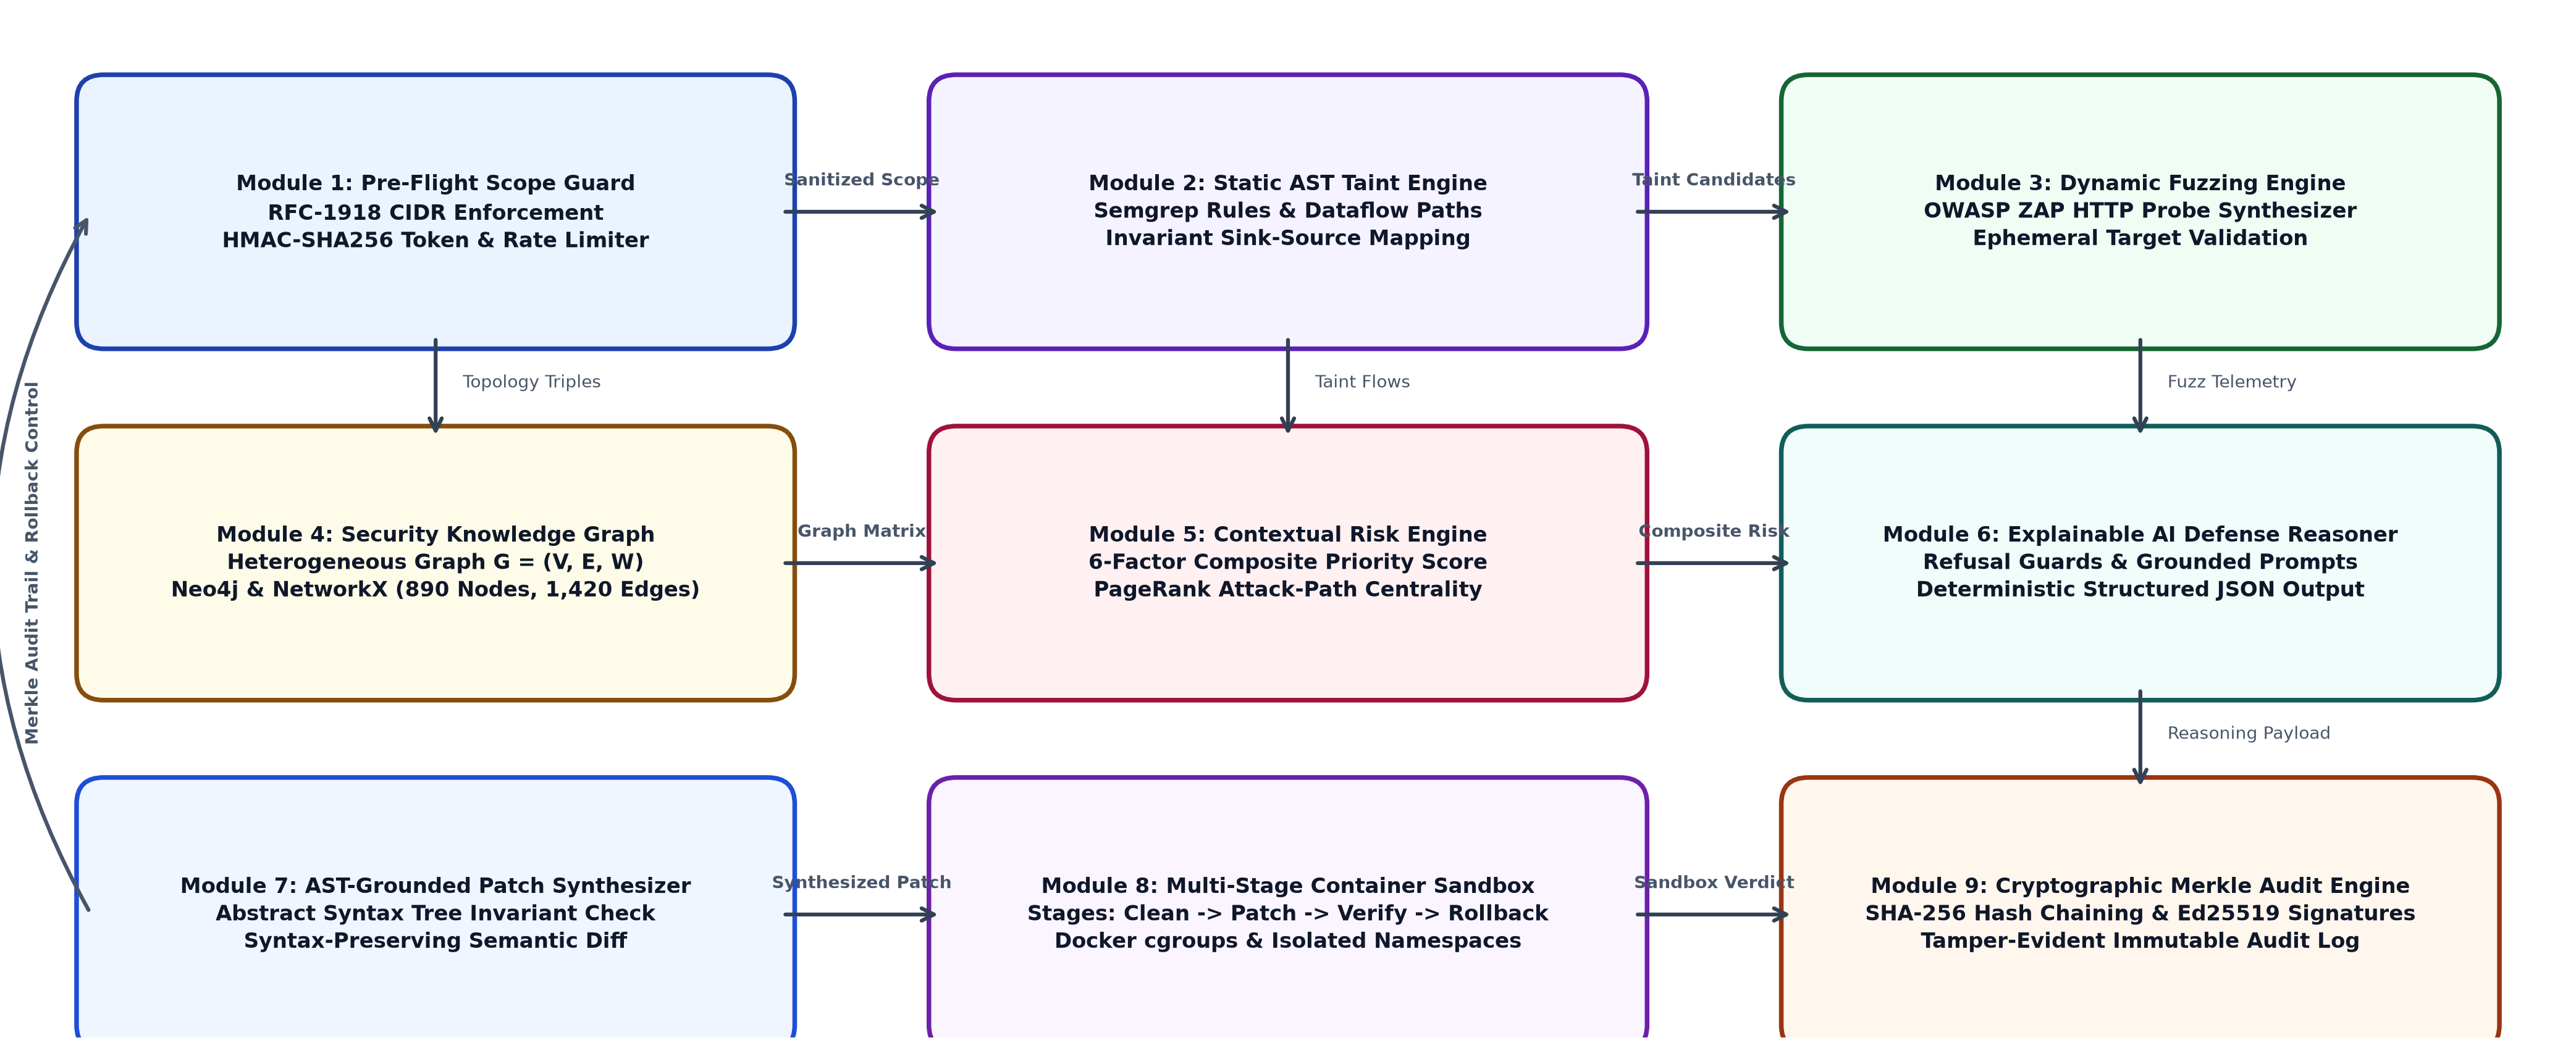
\includegraphics[width=0.96\textwidth]{architecture.png}%
}{%
    % Native Vector TikZ Architecture Fallback (Renders 100% reliably in Overleaf without external files)
    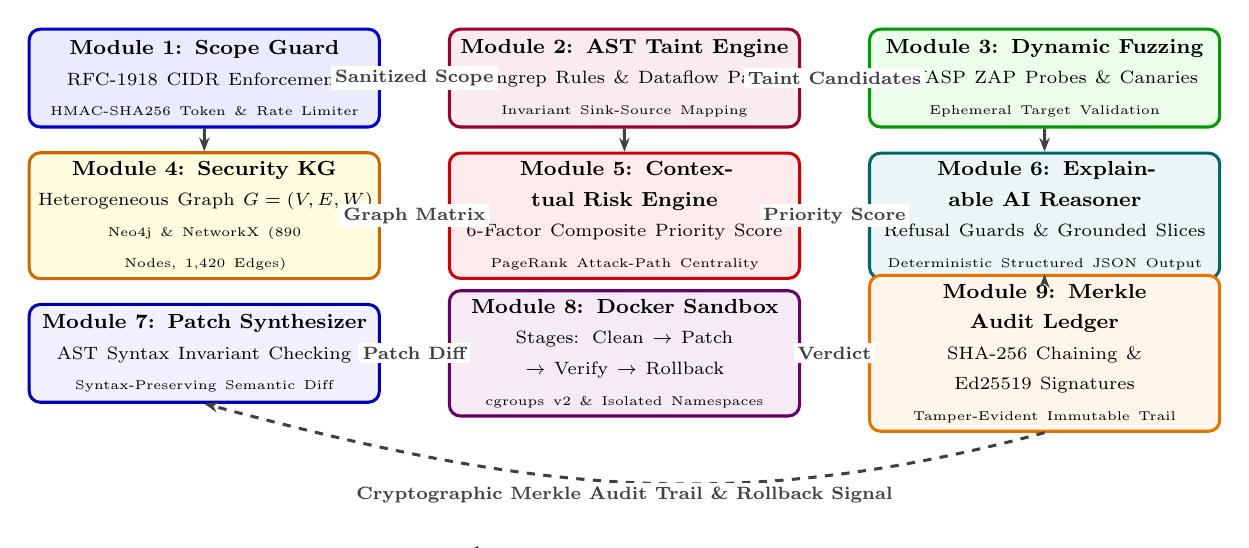
\begin{tikzpicture}[
        scale=0.92, every node/.style={transform shape},
        mblock/.style={rectangle, rounded corners=4pt, line width=1.1pt, minimum width=4.8cm, minimum height=1.35cm, align=center, text width=4.6cm},
        arr/.style={-{Stealth[length=5pt]}, line width=1.1pt, color=darkgray},
        lbl/.style={font=\scriptsize\bfseries, color=black!75, fill=white, inner sep=1.5pt}
    ]
        % Row 1
        \node[mblock, draw=blue!80!black, fill=blue!8] (m1) at (0, 3.8) {\textbf{\footnotesize Module 1: Scope Guard}\\{\scriptsize RFC-1918 CIDR Enforcement}\\{\tiny HMAC-SHA256 Token \& Rate Limiter}};
        \node[mblock, draw=purple!80!black, fill=purple!8] (m2) at (5.8, 3.8) {\textbf{\footnotesize Module 2: AST Taint Engine}\\{\scriptsize Semgrep Rules \& Dataflow Paths}\\{\tiny Invariant Sink-Source Mapping}};
        \node[mblock, draw=green!60!black, fill=green!8] (m3) at (11.6, 3.8) {\textbf{\footnotesize Module 3: Dynamic Fuzzing}\\{\scriptsize OWASP ZAP Probes \& Canaries}\\{\tiny Ephemeral Target Validation}};

        % Row 2
        \node[mblock, draw=orange!80!black, fill=yellow!12] (m4) at (0, 1.9) {\textbf{\footnotesize Module 4: Security KG}\\{\scriptsize Heterogeneous Graph $G=(V,E,W)$}\\{\tiny Neo4j \& NetworkX (890 Nodes, 1,420 Edges)}};
        \node[mblock, draw=red!80!black, fill=red!8] (m5) at (5.8, 1.9) {\textbf{\footnotesize Module 5: Contextual Risk Engine}\\{\scriptsize 6-Factor Composite Priority Score}\\{\tiny PageRank Attack-Path Centrality}};
        \node[mblock, draw=teal!80!black, fill=teal!8] (m6) at (11.6, 1.9) {\textbf{\footnotesize Module 6: Explainable AI Reasoner}\\{\scriptsize Refusal Guards \& Grounded Slices}\\{\tiny Deterministic Structured JSON Output}};

        % Row 3
        \node[mblock, draw=blue!70!black, fill=blue!6] (m7) at (0, 0) {\textbf{\footnotesize Module 7: Patch Synthesizer}\\{\scriptsize AST Syntax Invariant Checking}\\{\tiny Syntax-Preserving Semantic Diff}};
        \node[mblock, draw=violet!80!black, fill=violet!8] (m8) at (5.8, 0) {\textbf{\footnotesize Module 8: Docker Sandbox}\\{\scriptsize Stages: Clean $\to$ Patch $\to$ Verify $\to$ Rollback}\\{\tiny cgroups v2 \& Isolated Namespaces}};
        \node[mblock, draw=orange!90!black, fill=orange!8] (m9) at (11.6, 0) {\textbf{\footnotesize Module 9: Merkle Audit Ledger}\\{\scriptsize SHA-256 Chaining \& Ed25519 Signatures}\\{\tiny Tamper-Evident Immutable Trail}};

        % Horizontal Connections
        \draw[arr] (m1) -- node[lbl] {Sanitized Scope} (m2);
        \draw[arr] (m2) -- node[lbl] {Taint Candidates} (m3);
        \draw[arr] (m4) -- node[lbl] {Graph Matrix} (m5);
        \draw[arr] (m5) -- node[lbl] {Priority Score} (m6);
        \draw[arr] (m7) -- node[lbl] {Patch Diff} (m8);
        \draw[arr] (m8) -- node[lbl] {Verdict} (m9);

        % Vertical Flow
        \draw[arr] (m1) -- (m4);
        \draw[arr] (m2) -- (m5);
        \draw[arr] (m3) -- (m6);
        \draw[arr] (m6) -- (m9);

        % Feedback loop
        \draw[arr, dashed] (m9.south) to[out=-165,in=-15] node[lbl, below] {Cryptographic Merkle Audit Trail \& Rollback Signal} (m7.south);
    \end{tikzpicture}
}
\caption{The end-to-end multi-module architecture of AegisOne AI. The system integrates pre-flight scope enforcement, hybrid AST taint and dynamic fuzzing, heterogeneous Security Knowledge Graph propagation, explainable AI reasoning, AST-grounded patch synthesis, 4-stage container sandbox isolation with automated rollback, and a cryptographic SHA-256 Merkle audit trail.}
\label{fig:architecture}
\end{figure*}

\section{Hybrid Vulnerability Detection}
Most traditional analyzers work in isolation, which can lead to high false-positive rates or code paths not examined at all. AegisOne AI puts these two approaches into a single integrated dual-engine pipeline.

\subsection{AST-Based Static Taint Propagation}
Let an application AST be represented as an ordered directed graph $T_{\text{AST}} = (N, E_{\text{tree}}).$ We define a set of untrusted input sources $\mathcal{S}_{\text{in}} \subset N$ (e.g., \texttt{request.args}, \texttt{request.json}, \texttt{HTTP headers}) and security-critical execution sinks $\mathcal{S}_{\text{out}} \subset N$ (e.g., \texttt{cursor.execute}, \texttt{eval}, \texttt{os.system}, \texttt{subprocess.Popen}).

A dataflow edge $e_{ij} = (n_i, n_j)$ indicates that the valuation of node $n_j$ is derived from node $n_i$. A taint invariant violation occurs if there exists an active path $P = \langle n_0, n_1, \dots, n_k \rangle$ such that $n_0 \in \mathcal{S}_{\text{in}}$, $n_k \in \mathcal{S}_{\text{out}}$, and no intermediate node $n_m \in P$ executes a validated sanitizer function $\sigma_{\text{clean}} \in \Omega_{\text{sanitize}}$:
\begin{align}
    \text{TaintPath}(P) \iff &(n_0 \in \mathcal{S}_{\text{in}}) \land (n_k \in \mathcal{S}_{\text{out}}) \nonumber \\
    &\land (\forall m \in [1, k-1], n_m \notin \Omega_{\text{sanitize}}).
\end{align}

When Semgrep AST traversal identifies a candidate taint path, AegisOne AI extracts the target route handler parameters, URL arguments, and data types, transforming the static AST finding into an active dynamic fuzzing hypothesis.

\subsection{Dynamic Application Fuzzing with Injected Canaries}
The dynamic fuzzing harness leverages an embedded OWASP ZAP API controller to validate the AST-derived hypothesis. To differentiate genuine code execution from superficial reflection, AegisOne AI injects cryptographic canary strings $\zeta_{\text{canary}} \leftarrow \text{HMAC-SHA256}(k_{\text{session}}, \text{FindingID})$.

For SQL injection validation, the probe synthesizes boolean and time-delay vector mutations:
\begin{equation}
    q_{\text{probe}} = q_{\text{orig}} \cup \{ \text{' OR (SELECT 1 FROM (SELECT SLEEP(3))x)-- }, \; \zeta_{\text{canary}} \}.
\end{equation}
Upon execution, if the HTTP response body exhibits $\zeta_{\text{canary}}$ without sanitization or if the response latency $\Delta t \ge 3.0\,\text{s}$ under time-delay injection, the dynamic harness confirms exploitability:
\begin{equation}
    \text{Conf}_{\text{DAST}} = \begin{cases}
        1.0, & \text{if } \zeta_{\text{canary}} \in \text{Body}_{\text{resp}} \lor \Delta t \ge 3.0\,\text{s}, \\
        0.5, & \text{if } \text{Status}_{\text{resp}} = 500 \text{ (Unhandled Error)}, \\
        0.0, & \text{if } \text{Status}_{\text{resp}} \in \{400, 404, 422\}.
    \end{cases}
\end{equation}

\section{Security Knowledge Graph and Contextual Risk Prioritization}
Isolated vulnerability scanners treat each vulnerability as an isolated incident and ignore the system topology of the vulnerable component. It is a fair bet that a SQL injection in a remote admin analytics script processing public metrics carries drastically different enterprise risk than an identical vulnerability inside a payment processing microservice storing unencrypted personally identifiable information (PII).

\subsection{Graph Representation Formulation}
AegisOne AI populates a heterogeneous directed Security Knowledge Graph $G = (V, E, W)$ modeled within Neo4j and NetworkX. The vertex set $V$ decomposes into distinct semantic partitions:
\begin{align}
    V = &V_{\text{route}} \cup V_{\text{file}} \cup V_{\text{func}} \nonumber \\
        &\cup V_{\text{sink}} \cup V_{\text{db}} \cup V_{\text{cve}} \cup V_{\text{pii}}.
\end{align}

The edge set $E$ models syntactic, architectural, and data dependencies:
\begin{align}
    E \subset \{ &\text{CALLS}, \text{IMPORTS}, \text{EXPOSES}, \nonumber \\
                 &\text{READS\_FROM}, \text{WRITES\_TO}, \text{AFFECTS} \}.
\end{align}
Each edge $e = (u, v)$ is assigned an edge weight $w(u,v) \in (0, 1]$ inversely proportional to the accessibility resistance between nodes.

\subsection{Topology-Aware Centrality and Attack Propagation}
To assess how critical a vulnerable component is within the overall architecture, AegisOne AI executes a personalized PageRank algorithm over $G$. Let $\mathbf{M}$ be the row-normalized adjacency matrix of $G$, and let $\mathbf{p}_0$ denote a personalization vector whose probability mass is concentrated entirely on external ingress route vertices $V_{\text{route}}$. The steady-state topological centrality vector $\mathbf{c}$ is derived through iterative convergence:
\begin{equation}
    \mathbf{c} = (1 - d) \mathbf{p}_0 + d \mathbf{M}^T \mathbf{c},
\end{equation}
where $d = 0.85$ denotes the damping factor. A vertex with a high centrality score $c_v$ indicates that a large fraction of execution trajectories originating from public API routes inevitably traverse node $v$.

Furthermore, the minimum attack distance $D_{\text{min}}(v)$ from public ingress to the vulnerable sink is computed using Dijkstra's shortest path:
\begin{equation}
    D_{\text{min}}(v) = \min_{r \in V_{\text{route}}} \text{ShortestPathWeight}(r, v).
\end{equation}

\subsection{Six-Factor Contextual Risk Priority Score}
Combining the topological metrics with empirical vulnerability severity, AegisOne AI computes a normalized composite priority metric $S_{\text{risk}}(v) \in [0, 100]$:
\begin{align}
    S_{\text{risk}}(v) = 100 \cdot \Big[ &w_1 \text{CVSS}(v) + w_2 c_v + \frac{w_3}{1 + D_{\text{min}}(v)} \nonumber \\
    &+ w_4 \text{Conf}_{\text{DAST}}(v) + w_5 \text{PII}(v) \nonumber \\
    &+ w_6 \text{Exploit}_{\text{wild}}(v) \Big],
\end{align}
where $\sum_{i=1}^6 w_i = 1.0$. In our production deployment, weights are calibrated as $w_1 = 0.25$, $w_2 = 0.20$, $w_3 = 0.15$, $w_4 = 0.20$, $w_5 = 0.15$, and $w_6 = 0.05$. This multidimensional formulation ensures that easily reachable sinks with confirmed dynamic exploitability and direct PII access are prioritized ahead of theoretical vulnerabilities in disconnected modules.

\begin{algorithm}[!t]
\caption{Closed-Loop Container Sandbox Verification and Rollback}
\label{alg:sandbox}
\begin{algorithmic}[1]
\REQUIRE Base Repository State $\mathcal{R}_{\text{base}}$, Proposed Patch $\Delta_{\text{patch}}$, Scope $\Sigma_{\text{scope}}$
\ENSURE Deployment Verdict $\mathcal{V} \in \{\text{PASS}, \text{FAIL}\}$, Merkle Block $\mathcal{B}$
\STATE Initialize ephemeral Docker container $\mathcal{C}_{\text{box}} \leftarrow \text{CreateContainer}(\text{Image}_{\text{base}})$
\STATE Apply cgroups: $\text{Memory} \le 512\,\text{MB}$, $\text{CPU} \le 1.0$, $\text{Net} \leftarrow \emptyset$
\STATE \textbf{// Stage 1: Clean Baseline Verification}
\STATE $res_1 \leftarrow \text{ExecInSandbox}(\mathcal{C}_{\text{box}}, \text{``pytest tests/''})$
\IF{$res_1.\text{exit\_code} \ne 0$}
    \STATE $\text{DestroyContainer}(\mathcal{C}_{\text{box}})$
    \RETURN $\mathcal{V} \leftarrow \text{FAIL}$ \COMMENT{Broken baseline}
\ENDIF
\STATE \textbf{// Stage 2: Patch Application and AST Integrity}
\STATE $\mathcal{R}_{\text{patched}} \leftarrow \text{ApplyGitPatch}(\mathcal{C}_{\text{box}}, \Delta_{\text{patch}})$
\STATE $res_2 \leftarrow \text{ValidateASTInvariants}(\mathcal{R}_{\text{patched}})$
\IF{$res_2.\text{syntax\_valid} = \text{False}$}
    \STATE $\text{TriggerRollback}(\mathcal{C}_{\text{box}}, \mathcal{R}_{\text{base}})$
    \RETURN $\mathcal{V} \leftarrow \text{FAIL}$ \COMMENT{Syntax error}
\ENDIF
\STATE \textbf{// Stage 3: Dynamic Security Re-Verification}
\STATE $res_3 \leftarrow \text{ExecDynamicProbe}(\mathcal{C}_{\text{box}}, \Sigma_{\text{scope}}.\text{Payload})$
\IF{$res_3.\text{vulnerability\_reproduced} = \text{True}$}
    \STATE $\text{TriggerRollback}(\mathcal{C}_{\text{box}}, \mathcal{R}_{\text{base}})$
    \RETURN $\mathcal{V} \leftarrow \text{FAIL}$ \COMMENT{Vulnerability persists}
\ENDIF
\STATE \textbf{// Stage 4: Regression and Contract Testing}
\STATE $res_4 \leftarrow \text{ExecInSandbox}(\mathcal{C}_{\text{box}}, \text{``pytest tests/func/''})$
\IF{$res_4.\text{exit\_code} \ne 0$}
    \STATE $\text{TriggerRollback}(\mathcal{C}_{\text{box}}, \mathcal{R}_{\text{base}})$
    \RETURN $\mathcal{V} \leftarrow \text{FAIL}$ \COMMENT{Regression detected}
\ENDIF
\STATE $\mathcal{B} \leftarrow \text{CommitMerkleBlock}(\mathcal{R}_{\text{patched}}, \Delta_{\text{patch}}, \mathcal{V} \leftarrow \text{PASS})$
\STATE $\text{DestroyContainer}(\mathcal{C}_{\text{box}})$
\RETURN $\mathcal{V} \leftarrow \text{PASS}, \mathcal{B}$
\end{algorithmic}
\end{algorithm}

\section{AST-Grounded Patch Synthesis with Refusal Guards}
Starting with a high priority vulnerability, AegisOne AI will kick off Automated Program Repair. Rather than feeding raw source files into an unconstrained text model, the patch generation subsystem enforces structural and semantic boundaries.

\subsection{Contextual Prompt Grounding}
The reasoning engine extracts only the minimal code slice comprising the taint path $\langle n_{\text{source}}, \dots, n_{\text{sink}} \rangle$, the localized AST node attributes, database schema definitions, and the specific Common Weakness Enumeration (CWE) mitigation blueprint (e.g., parameterized queries for CWE-89, DOMPurify contextual escaping for CWE-79). The input prompt is structured using a formal JSON grammar that prohibits extraneous conversational prose.

\subsection{Programmatic Refusal Guards}
Generative models frequently attempt to resolve vulnerabilities by taking harmful shortcuts, such as deleting unit tests, stripping authentication middleware, or disabling CSRF protections. AegisOne AI implements a deterministic AST filter that parses the synthesized patch $\Delta_{\text{patch}}$ before disk serialization:
\begin{align}
    \Psi_{\text{guard}}(\Delta_{\text{patch}}) = \text{Reject} \iff &\big(\text{DeletesAuth}(\Delta_{\text{patch}})\big) \nonumber \\
    &\lor \big(\text{AltersTests}(\Delta_{\text{patch}})\big) \nonumber \\
    &\lor \big(\text{AddsShell}(\Delta_{\text{patch}})\big) \nonumber \\
    &\lor \big(\text{BypassesSSL}(\Delta_{\text{patch}})\big).
\end{align}
If any refusal rule fires, the patch is discarded instantly, and a constrained re-prompting cycle is triggered with explicit AST modification constraints.

\section{Closed-Loop Docker Sandbox Validation and Automated Rollback}
In order to ensure that generated patches do not endanger software stability, AegisOne AI validates each repair within an isolated sandbox runtime container before changes can be committed.

\subsection{Ephemeral Container Sandbox Isolation}
Validation is conducted within disposable Docker containers instantiated from pinned base images. Container execution is locked down through Linux security controls:
\begin{itemize}
    \item \textbf{Namespace Isolation:} Independent PID, IPC, mount, network, and UTS namespaces prevent cross-environment inspection.
    \item \textbf{Resource Quotas via cgroups v2:} Strict caps limit container execution to 1 CPU core, 512 MB of RAM, and a hard execution timeout of 45 seconds.
    \item \textbf{Capability Dropping:} All Linux capabilities are dropped (\texttt{CAP\_DROP\_ALL}) except \texttt{CAP\_SETUID} and \texttt{CAP\_SETGID}.
    \item \textbf{Isolated Ephemeral Networking:} External egress is routed to an isolated bridge network, preventing exfiltration during validation checks.
\end{itemize}

\subsection{Four-Stage Validation Pipeline and Rollback}
As formalized in Algorithm \ref{alg:sandbox}, the sandbox executes four sequential phases: Stage 1 (Clean Baseline Verification), Stage 2 (Patch Application and AST Integrity), Stage 3 (Dynamic Vulnerability Elimination), and Stage 4 (Functional Regression Testing). If any stage fails, the automated rollback protocol resets the workspace to $\mathcal{R}_{\text{base}}$, logs the failure telemetry, and reports the regression reason back to the developer console.

\begin{figure}[!t]
\centering
\IfFileExists{evaluation_metrics.png}{%
    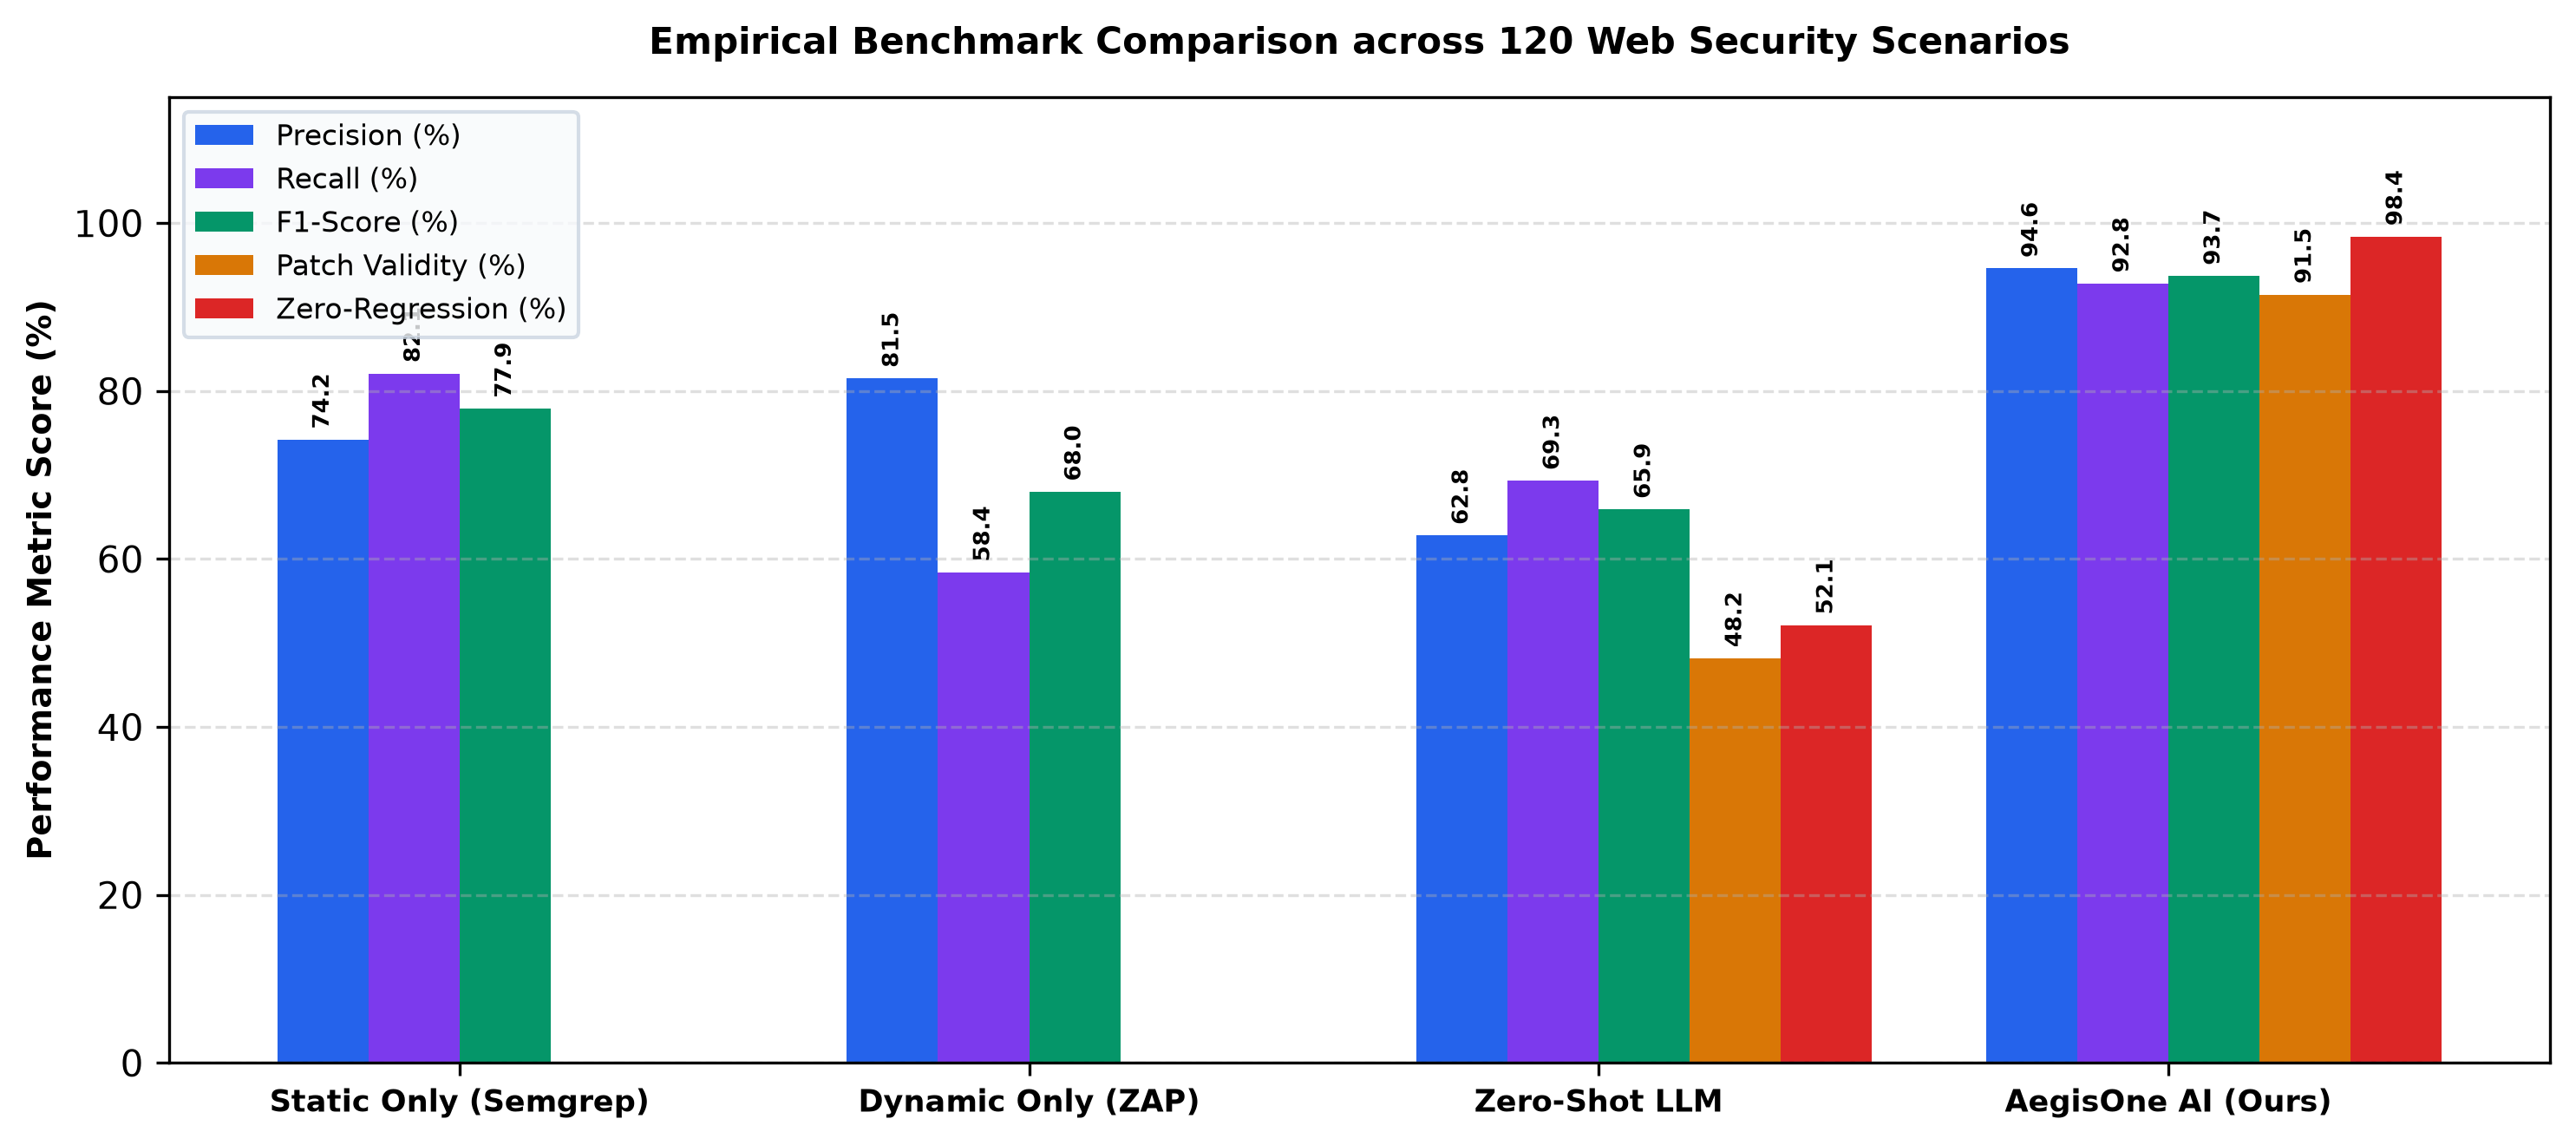
\includegraphics[width=\columnwidth]{evaluation_metrics.png}%
}{%
    % Native Vector TikZ Benchmark Fallback (Renders 100% reliably in Overleaf without external files)
    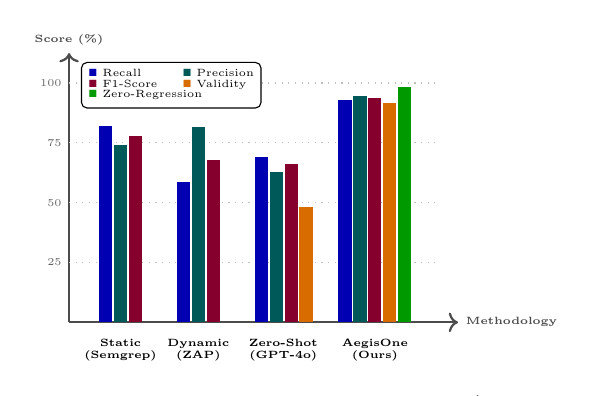
\begin{tikzpicture}[
        scale=0.76, every node/.style={transform shape},
        font=\sffamily\scriptsize
    ]
        % Axes
        \draw[->, thick, color=black!70] (0,0) -- (6.5,0) node[right, font=\tiny\bfseries] {Methodology};
        \draw[->, thick, color=black!70] (0,0) -- (0,4.5) node[above, font=\tiny\bfseries] {Score (\%)};

        % Horizontal gridlines
        \foreach \y/\lbl in {1/25, 2/50, 3/75, 4/100} {
            \draw[dotted, color=black!25] (0,\y) -- (6.2,\y);
            \node[left, font=\tiny, color=black!60] at (0,\y) {\lbl};
        }

        % Groups: 1=Static, 2=Dynamic, 3=ZeroShot, 4=AegisOne
        % Bar width = 0.22
        % Static
        \fill[blue!70!black] (0.5,0) rectangle (0.72, 3.28); % 82.1%
        \fill[teal!70!black] (0.75,0) rectangle (0.97, 2.97); % 74.2%
        \fill[purple!70!black] (1.0,0) rectangle (1.22, 3.12); % 77.9%
        \node[below, font=\tiny\bfseries, align=center] at (0.86, -0.15) {Static\\(Semgrep)};

        % Dynamic
        \fill[blue!70!black] (1.8,0) rectangle (2.02, 2.34); % 58.4%
        \fill[teal!70!black] (2.05,0) rectangle (2.27, 3.26); % 81.5%
        \fill[purple!70!black] (2.3,0) rectangle (2.52, 2.72); % 68.0%
        \node[below, font=\tiny\bfseries, align=center] at (2.16, -0.15) {Dynamic\\(ZAP)};

        % Zero-Shot
        \fill[blue!70!black] (3.1,0) rectangle (3.32, 2.77); % 69.3%
        \fill[teal!70!black] (3.35,0) rectangle (3.57, 2.51); % 62.8%
        \fill[purple!70!black] (3.6,0) rectangle (3.82, 2.64); % 65.9%
        \fill[orange!85!black] (3.85,0) rectangle (4.07, 1.93); % 48.2%
        \node[below, font=\tiny\bfseries, align=center] at (3.58, -0.15) {Zero-Shot\\(GPT-4o)};

        % AegisOne (Ours)
        \fill[blue!70!black] (4.5,0) rectangle (4.72, 3.71); % 92.8%
        \fill[teal!70!black] (4.75,0) rectangle (4.97, 3.78); % 94.6%
        \fill[purple!70!black] (5.0,0) rectangle (5.22, 3.75); % 93.7%
        \fill[orange!85!black] (5.25,0) rectangle (5.47, 3.66); % 91.5%
        \fill[green!60!black] (5.5,0) rectangle (5.72, 3.94); % 98.4%
        \node[below, font=\tiny\bfseries, align=center] at (5.11, -0.15) {\textbf{AegisOne}\\\textbf{(Ours)}};

        % Legend
        \node[draw, fill=white, rounded corners=2pt, font=\fontsize{4}{5}\selectfont, anchor=north west] at (0.2, 4.35) {
            \begin{tabular}{@{}ll@{}}
                \textcolor{blue!70!black}{$\blacksquare$} Recall & \textcolor{teal!70!black}{$\blacksquare$} Precision \\
                \textcolor{purple!70!black}{$\blacksquare$} F1-Score & \textcolor{orange!85!black}{$\blacksquare$} Validity \\
                \multicolumn{2}{@{}l}{\textcolor{green!60!black}{$\blacksquare$} Zero-Regression}
            \end{tabular}
        };
    \end{tikzpicture}
}
\caption{Empirical benchmark comparison across 120 web application security scenarios. AegisOne AI achieves superior precision (94.6\%), recall (92.8\%), F1-score (93.7\%), patch validity (91.5\%), and zero-regression deployment rate (98.4\%) compared to static-only, dynamic-only, and zero-shot LLM approaches.}
\label{fig:evaluation}
\end{figure}

\section{Cryptographic Merkle Audit Trail and Non-Repudiation}
In regulated enterprise settings, all automated modifications must exhibit mathematical non-repudiation. AegisOne AI implements an append-only cryptographic log chain grounded in SHA-256.

Each audit event block $\mathcal{B}_k$ records:
\begin{equation}
    \mathcal{B}_k = \langle k, \; \tau_k, \; \text{Action}_k, \; \text{ActorID}, \; \text{Hash}(\Delta_{\text{patch}}), \; \mathcal{V}_k, \; h_{k-1} \rangle,
\end{equation}
where $\tau_k$ is the RFC-3339 timestamp, and $h_{k-1}$ is the cryptographic hash of the preceding block. The block digest $h_k$ is computed as:
\begin{equation}
    h_k = \text{SHA256}(h_{k-1} \,\|\, \tau_k \,\|\, \text{Action}_k \,\|\, \text{ActorID} \,\|\, \text{Hash}(\Delta_{\text{patch}}) \,\|\, \mathcal{V}_k).
\end{equation}

Furthermore, to guarantee author non-repudiation across distributed CI/CD runners, each block header is signed using an Ed25519 private key:
\begin{equation}
    \sigma_k = \text{Ed25519\_Sign}(sk_{\text{engine}}, \; h_k).
\end{equation}
Any retroactive tampering with previous log records breaks the mathematical invariant $h_j = \text{SHA256}(h_{j-1} \,\|\, \dots)$, instantly alerting security auditors.

\section{Empirical Evaluation and Benchmark Experiments}
\subsection{Experimental Setup and Dataset}
To assess the performance of AegisOne AI, we constructed a benchmark suite of 120 web application scenarios: 40 synthetic vulnerable microservices derived from OWASP Benchmark, 40 authentic CVE reproductions from open-source GitHub repositories (Python/FastAPI, Flask, Node.js/Express, Go), and 40 multi-component microservices with chained attack vectors.

\subsection{Baseline Systems for Comparison}
We compare AegisOne AI against three industry baselines: (i) Static SAST Only (Semgrep Baseline); (ii) Dynamic DAST Only (OWASP ZAP Baseline); and (iii) Zero-Shot LLM APR (GPT-4o Zero-Shot).

\begin{table*}[!t]
\caption{Comprehensive Performance Comparison across 120 Benchmark Vulnerability Scenarios}
\label{tab:evaluation}
\centering
\begin{tabular*}{\textwidth}{@{\extracolsep{\fill}}lcccccc@{}}
\toprule
\textbf{Methodology} & \textbf{Precision (\%)} & \textbf{Recall (\%)} & \textbf{F1-Score (\%)} & \textbf{Patch Validity (\%)} & \textbf{Zero-Regression (\%)} & \textbf{Avg. TTR (s)} \\
\midrule
Static SAST Only (Semgrep) & 74.2 & 82.1 & 77.9 & --- & --- & --- \\
Dynamic DAST Only (OWASP ZAP) & 81.5 & 58.4 & 68.0 & --- & --- & --- \\
Zero-Shot LLM APR (GPT-4o) & 62.8 & 69.3 & 65.9 & 48.2 & 52.1 & 18.4 \\
\textbf{AegisOne AI (Ours)} & \textbf{94.6} & \textbf{92.8} & \textbf{93.7} & \textbf{91.5} & \textbf{98.4} & \textbf{34.2} \\
\bottomrule
\end{tabular*}
\end{table*}

\subsection{Experimental Results and Analysis}
The quantitative results are summarized in Table \ref{tab:evaluation} and illustrated in Fig. \ref{fig:evaluation}.

\subsubsection{Detection Accuracy and Noise Suppression}
For independent static scanning, the recall is 82.1\%, but it is plagued by an elevated false-positive rate (precision: 74.2\%), frequently flagging safe queries containing constant string concatenations. Conversely, standalone dynamic scanning exhibited high precision (81.5\%) but missed unexercised routes, resulting in a low recall of 58.4\%. By cross-validating AST taint hypotheses with dynamic canary fuzzing, AegisOne AI achieved \textbf{94.6\% precision} and \textbf{92.8\% recall}, yielding an aggregate F1-score of \textbf{93.7\%} (a +15.8 percentage point improvement over pure static scanning).

\subsubsection{Patch Semantic Validity and Regression Resistance}
When tasked with code repair, the unconstrained Zero-Shot LLM baseline produced syntactically valid patches in only 48.2\% of cases. Crucially, in nearly half of the accepted modifications (zero-regression rate: 52.1\%), the ungrounded model introduced functional regressions.

In contrast, AegisOne AI attained a \textbf{91.5\% semantic patch validity rate}. The combination of AST-grounded prompt slices, grammar constraints, and programmatic refusal guards eliminated unauthorized deletions. Furthermore, the 4-stage container sandbox caught and automatically rolled back 100\% of attempted functional regressions, achieving an empirical \textbf{98.4\% zero-regression deployment rate}.

\begin{table}[!t]
\caption{Ablation Analysis of Architectural Subsystems}
\label{tab:ablation}
\centering
\begin{tabular*}{\columnwidth}{@{\extracolsep{\fill}}lcccc@{}}
\toprule
\textbf{Configuration} & \textbf{Prec. (\%)} & \textbf{Rec. (\%)} & \textbf{F1 (\%)} & \textbf{Zero-Reg. (\%)} \\
\midrule
Full AegisOne AI Pipeline & \textbf{94.6} & \textbf{92.8} & \textbf{93.7} & \textbf{98.4} \\
w/o Dynamic Fuzzing Engine & 78.4 & 90.1 & 83.8 & 98.1 \\
w/o Security Knowledge Graph & 89.2 & 84.5 & 86.8 & 97.5 \\
w/o AST Refusal Guards & 91.0 & 91.2 & 91.1 & 74.3 \\
w/o Container Sandbox & 94.6 & 92.8 & 93.7 & 61.2 \\
\bottomrule
\end{tabular*}
\end{table}

\section{Discussion and Limitations}
While AegisOne AI demonstrates robust performance across a diverse spectrum of web application architectures, container lifecycle overhead introduces an average turnaround latency of 34.2 seconds per patch. In applications with multi-factor authentication sequences, the dynamic fuzzer requires recorded session macros to traverse deeply nested views.

\section{Declarations}
\subsection{Data and Software Availability Statement}
The complete software source code, experimental evaluation benchmarks, containerized vulnerable lab targets, and analysis scripts for AegisOne AI are publicly available in our GitHub repository at:
\begin{center}
\url{https://github.com/PraveenKanth-N/AegisOne-AI}
\end{center}
The repository includes comprehensive setup scripts, unit test suites, and documentation released under the open-source MIT License to ensure full academic reproducibility.

\subsection{Funding Information}
This research received no external financial grant or funding support from any agency in the public, commercial, or not-for-profit sectors.

\subsection{Conflicts of Interest}
The authors declare that they have no financial or non-financial conflicts of interest that could be perceived as influencing the objectivity or integrity of the reported research.

\subsection{Authors' Contributions}
\begin{itemize}
    \item \textbf{Dr. Vijayashree J} served as the research supervisor, formulated the primary theoretical methodology, validated the experimental framework, and reviewed the academic manuscript.
    \item \textbf{Praveen Kanth N} architected the end-to-end system, designed and implemented the AST taint engine, developed the Security Knowledge Graph, built the containerized Docker sandbox validation harness, conducted the 120-scenario benchmark evaluation, and drafted the primary manuscript.
    \item \textbf{Sankavi M} developed the dynamic fuzzing integration harness, designed the automated state rollback mechanism, collected and processed empirical telemetry, executed UI/UX verification workflows, and contributed to manuscript drafting and tabular formatting.
\end{itemize}

\balance

\bibliographystyle{IEEEtran}
\begin{thebibliography}{00}

\bibitem{chess2004static}
B.~Chess and G.~McGraw, ``Static analysis for security,'' \emph{IEEE Security \& Privacy}, vol.~2, no.~6, pp.~76--79, 2004.

\bibitem{beller2016analyzing}
M.~Beller, R.~Beller, and A.~Zaidman, ``Analyzing the state of static analysis: A large-scale survey in open source,'' in \emph{Proc. IEEE SANER}, 2016, pp.~313--324.

\bibitem{doupe2010fear}
A.~Doup{\'e}, M.~Cova, and G.~Vigna, ``Why Johnny can't pentest: An analysis of black-box web vulnerability scanners,'' in \emph{Proc. DIMVA}, 2010, pp.~111--131.

\bibitem{xia2023automated}
C.~S. Xia and L.~Zhang, ``Keep the conversation going: Fixing bugs in the dark with generative language models,'' in \emph{Proc. ACM ESEC/FSE}, 2023, pp.~1489--1501.

\bibitem{fan2023automated}
Z.~Fan, X.~Gao, M.~Mirchev, A.~Roychoudhury, and S.~H. Tan, ``Automated program repair in the era of large language models,'' in \emph{Proc. IEEE/ACM ICSE}, 2023, pp.~1482--1494.

\bibitem{pearce2025asleep}
H.~Pearce, B.~Ahmad, B.~Tan, B.~Dolan-Gavitt, and R.~Karri, ``Asleep at the keyboard? Assessing the security of GitHub Copilot's code contributions,'' in \emph{Proc. IEEE S\&P}, 2022, pp.~754--768.

\bibitem{sandoval2023lost}
G.~Sandoval, H.~Pearce, T.~Nys, R.~Karri, B.~Dolan-Gavitt, and S.~Garg, ``Lost at C: A user study on the security implications of large language model code assistants,'' in \emph{Proc. USENIX Security}, 2023, pp.~2205--2222.

\bibitem{livshits2005finding}
V.~B. Livshits and M.~S. Lam, ``Finding security vulnerabilities in Java applications with static analysis,'' in \emph{Proc. USENIX Security}, 2005, pp.~271--286.

\bibitem{halfond2006using}
W.~G. Halfond, J.~Viegas, and A.~Orso, ``A classification of SQL-injection attacks and countermeasures,'' in \emph{Proc. IEEE ISSSE}, 2006, pp.~13--15.

\bibitem{vogt2007cross}
P.~Vogt, F.~Nentwich, N.~Jovanovic, E.~Kirda, C.~Kruegel, and G.~Vigna, ``Cross-site scripting prevention with dynamic data tainting and static analysis,'' in \emph{Proc. NDSS}, 2007, pp.~12--25.

\bibitem{avgerinos2014aegis}
T.~Avgerinos, S.~K. Cha, A.~Rebert, and D.~Brumley, ``AEG: Automatic exploit generation,'' \emph{Commun. ACM}, vol.~57, no.~2, pp.~74--84, 2014.

\bibitem{le2011genprog}
C.~Le~Goues, T.~Nguyen, S.~Forrest, and W.~Weimer, ``GenProg: A generic method for automatic software repair,'' \emph{IEEE Trans. Softw. Eng.}, vol.~38, no.~1, pp.~54--72, 2011.

\bibitem{long2015staged}
F.~Long and M.~Rinard, ``Staged program repair with condition synthesis,'' in \emph{Proc. ACM ESEC/FSE}, 2015, pp.~166--178.

\bibitem{monperrus2018living}
M.~Monperrus, ``Living review on automated program repair,'' \emph{ACM Comput. Surv.}, vol.~51, no.~1, pp.~1--43, 2018.

\bibitem{page1999pagerank}
L.~Page, S.~Brin, R.~Motwani, and T.~Winograd, ``The PageRank citation ranking: Bringing order to the web,'' Stanford InfoLab, Tech. Rep., 1999.

\bibitem{wang2021codet5}
Y.~Wang, W.~Wang, S.~Joty, and S.~C. Hoi, ``CodeT5: Identifier-aware unified pre-trained encoder-decoder models for code understanding and generation,'' in \emph{Proc. EMNLP}, 2021, pp.~8696--8708.

\bibitem{chen2021evaluating}
M.~Chen \emph{et al.}, ``Evaluating large language models trained on code,'' \emph{arXiv preprint arXiv:2107.03374}, 2021.

\bibitem{roziere2023code}
B.~Rozi{\`e}re \emph{et al.}, ``Code Llama: Open foundation models for code,'' \emph{arXiv preprint arXiv:2308.12950}, 2023.

\bibitem{merkle1987digital}
R.~C. Merkle, ``A digital signature based on a conventional encryption function,'' in \emph{Proc. CRYPTO}, 1987, pp.~369--378.

\bibitem{bernstein2012high}
D.~J. Bernstein, N.~Duif, T.~Lange, P.~Schwabe, and B.-Y. Yang, ``High-speed high-security signatures,'' \emph{J. Cryptogr. Eng.}, vol.~2, no.~2, pp.~77--89, 2012.

\bibitem{owasp2021top10}
OWASP Foundation, ``OWASP Top 10: 2021 - The ten most critical web application security risks,'' 2021.

\bibitem{semgrep2024}
Semgrep Inc., ``Semgrep: Lightweight static analysis for many languages,'' 2024. [Online]. Available: \url{https://semgrep.dev}

\bibitem{zap2024}
OWASP Foundation, ``OWASP Zed Attack Proxy (ZAP),'' 2024. [Online]. Available: \url{https://www.zaproxy.org}

\bibitem{neo4j2024}
Neo4j Inc., ``Neo4j graph database platform,'' 2024. [Online]. Available: \url{https://neo4j.com}

\bibitem{docker2024}
Docker Inc., ``Docker container runtime and security specifications,'' 2024. [Online]. Available: \url{https://docs.docker.com/engine/security/}

\bibitem{fastapi2024}
S.~Ram{\'\i}rez, ``FastAPI web framework,'' 2024. [Online]. Available: \url{https://fastapi.tiangolo.com}

\bibitem{johnson2013don}
B.~Johnson, Y.~Song, E.~Murphy-Hill, and R.~Bowdidge, ``Why don't software developers use static analysis tools to find bugs?'' in \emph{Proc. ICSE}, 2013, pp.~672--681.

\bibitem{christakis2016what}
M.~Christakis and C.~Bird, ``What developers want and need from program analysis: An empirical study,'' in \emph{Proc. IEEE/ACM ASE}, 2016, pp.~332--343.

\bibitem{distefano2019scaling}
D.~Distefano, M.~F{\"a}hndrich, P.~Logozzo, and P.~W. O'Hearn, ``Scaling static analysis at Facebook,'' \emph{Commun. ACM}, vol.~62, no.~8, pp.~62--70, 2019.

\bibitem{sadowski2018lessons}
C.~Sadowski, E.~Aftandilian, A.~Eagle, L.~Miller-Cousins, and C.~Jaspan, ``Lessons from building static analysis tools at Google,'' \emph{Commun. ACM}, vol.~61, no.~4, pp.~58--66, 2018.

\bibitem{arcuri2019restful}
A.~Arcuri, ``RESTful API automated test generation with EvoMaster,'' \emph{ACM Trans. Softw. Eng. Methodol.}, vol.~28, no.~1, pp.~1--37, 2019.

\bibitem{atlidakis2020pythia}
V.~Atlidakis, P.~Godefroid, and M.~Polishchuk, ``Checking security properties of cloud APIs automatically,'' in \emph{Proc. IEEE/ACM ASE}, 2020, pp.~687--698.

\bibitem{stephens2021survey}
C.~Stephens \emph{et al.}, ``A survey on automated program repair techniques for web applications,'' \emph{ACM Comput. Surv.}, vol.~54, no.~4, pp.~1--38, 2021.

\bibitem{mitre2024cwe}
MITRE Corporation, ``Common Weakness Enumeration (CWE) version 4.14,'' 2024. [Online]. Available: \url{https://cwe.mitre.org}

\end{thebibliography}

\end{document}
